% design-document.tex — CSEE 4840 Design Document: Plants vs Zombies on FPGA
\documentclass[11pt,letterpaper]{article}

% ── Layout ──────────────────────────────────────────────────────────────
\usepackage[margin=1in]{geometry}
\usepackage{fancyhdr}
\pagestyle{fancy}
\fancyhf{}
\lhead{CSEE 4840 --- Plants vs Zombies on FPGA}
\rhead{Spring 2026}
\cfoot{\thepage}

% ── Typography & Math ───────────────────────────────────────────────────
\usepackage{amsmath,amssymb}
\usepackage{enumitem}
\usepackage{parskip}

% ── Tables ──────────────────────────────────────────────────────────────
\usepackage{booktabs}
\usepackage{multirow}
\usepackage{tabularx}
\usepackage{array}

% ── Graphics & Color ────────────────────────────────────────────────────
\usepackage{graphicx}
\usepackage[dvipsnames,svgnames,x11names]{xcolor}
\usepackage{float}

% ── Code Listings ───────────────────────────────────────────────────────
\usepackage{listings}
\lstset{
  basicstyle=\ttfamily\small,
  keywordstyle=\bfseries\color{NavyBlue},
  commentstyle=\color{ForestGreen},
  frame=single,
  breaklines=true,
  numbers=left,
  numberstyle=\tiny\color{gray},
  xleftmargin=2em,
  framexleftmargin=1.5em,
}

% ── TikZ ────────────────────────────────────────────────────────────────
\usepackage{tikz}
\usetikzlibrary{
  arrows.meta,
  positioning,
  shapes.geometric,
  shapes.multipart,
  calc,
  decorations.pathreplacing,
  fit,
  backgrounds,
  patterns,
}

% ── Hyperlinks ──────────────────────────────────────────────────────────
\usepackage[colorlinks=true,linkcolor=NavyBlue,urlcolor=RoyalBlue]{hyperref}

% ── Custom column types ─────────────────────────────────────────────────
\newcolumntype{C}[1]{>{\centering\arraybackslash}p{#1}}
\newcolumntype{L}[1]{>{\raggedright\arraybackslash}p{#1}}
\newcolumntype{R}[1]{>{\raggedleft\arraybackslash}p{#1}}

% ════════════════════════════════════════════════════════════════════════
\begin{document}

% ── Title ───────────────────────────────────────────────────────────────
\begin{center}
  {\LARGE\bfseries Plants vs Zombies on FPGA}\\[0.6em]
  {\large CSEE 4840 Embedded System Design --- Spring 2026}\\[1.2em]
  \begin{tabular}{llll}
    Hao Cai & \texttt{hc3612} &
    Chenhao Yang & \texttt{cy2822} \\
    Zhenghang Zhao & \texttt{zz3410} &
    Yabkun Li & \texttt{yl6022} \\
  \end{tabular}
\end{center}

\tableofcontents
\newpage

% ════════════════════════════════════════════════════════════════════════
\section{Introduction}
\label{sec:intro}

We are building a simplified version of \emph{Plants vs Zombies} on the
Terasic DE1-SoC board. The game takes place on a $5 \times 9$ grid where
the player places defensive plants to stop waves of zombies that walk in
from the right edge of the screen. Surviving every wave wins the game;
letting a single zombie reach the left edge loses it.

The work divides between hardware and software along the HPS--FPGA
boundary. The FPGA drives a 640$\times$480 VGA display at 60\,Hz
through a scanline-based pipeline with dual line buffers and a
shape/sprite table. The HPS runs Linux and hosts the game loop in C:
grid state management, plant and zombie logic, collision detection, the
sun resource economy, and input polling from a USB gamepad via
\texttt{libusb}. A kernel driver sits between the two, exposing
memory-mapped Avalon registers as \texttt{ioctl} calls on
\texttt{/dev/pvz}.

Audio goes through the on-board Wolfson WM8731 codec. We plan to stream
an 8-bit PCM arrangement of the Plants vs Zombies theme as background
music, with short sound effects (pea fire, zombie groan, plant placement)
mixed on top.

The rest of this document covers the system architecture, algorithms on
both sides of the HPS--FPGA boundary, resource budgets, and a bit-level
specification of the control registers.

% ════════════════════════════════════════════════════════════════════════
\section{System Block Diagram}
\label{sec:blockdiag}

Figure~\ref{fig:system-block} shows the full system. The left half runs
on the ARM Cortex-A9 under Linux; the right half is synthesized into the
FPGA fabric. Communication crosses a single lightweight AXI bridge that
the Avalon-MM agent sits behind, mapped at physical address
\texttt{0xFF200000} from the CPU's perspective.

\begin{figure}[H]
\centering
\resizebox{\textwidth}{!}{%
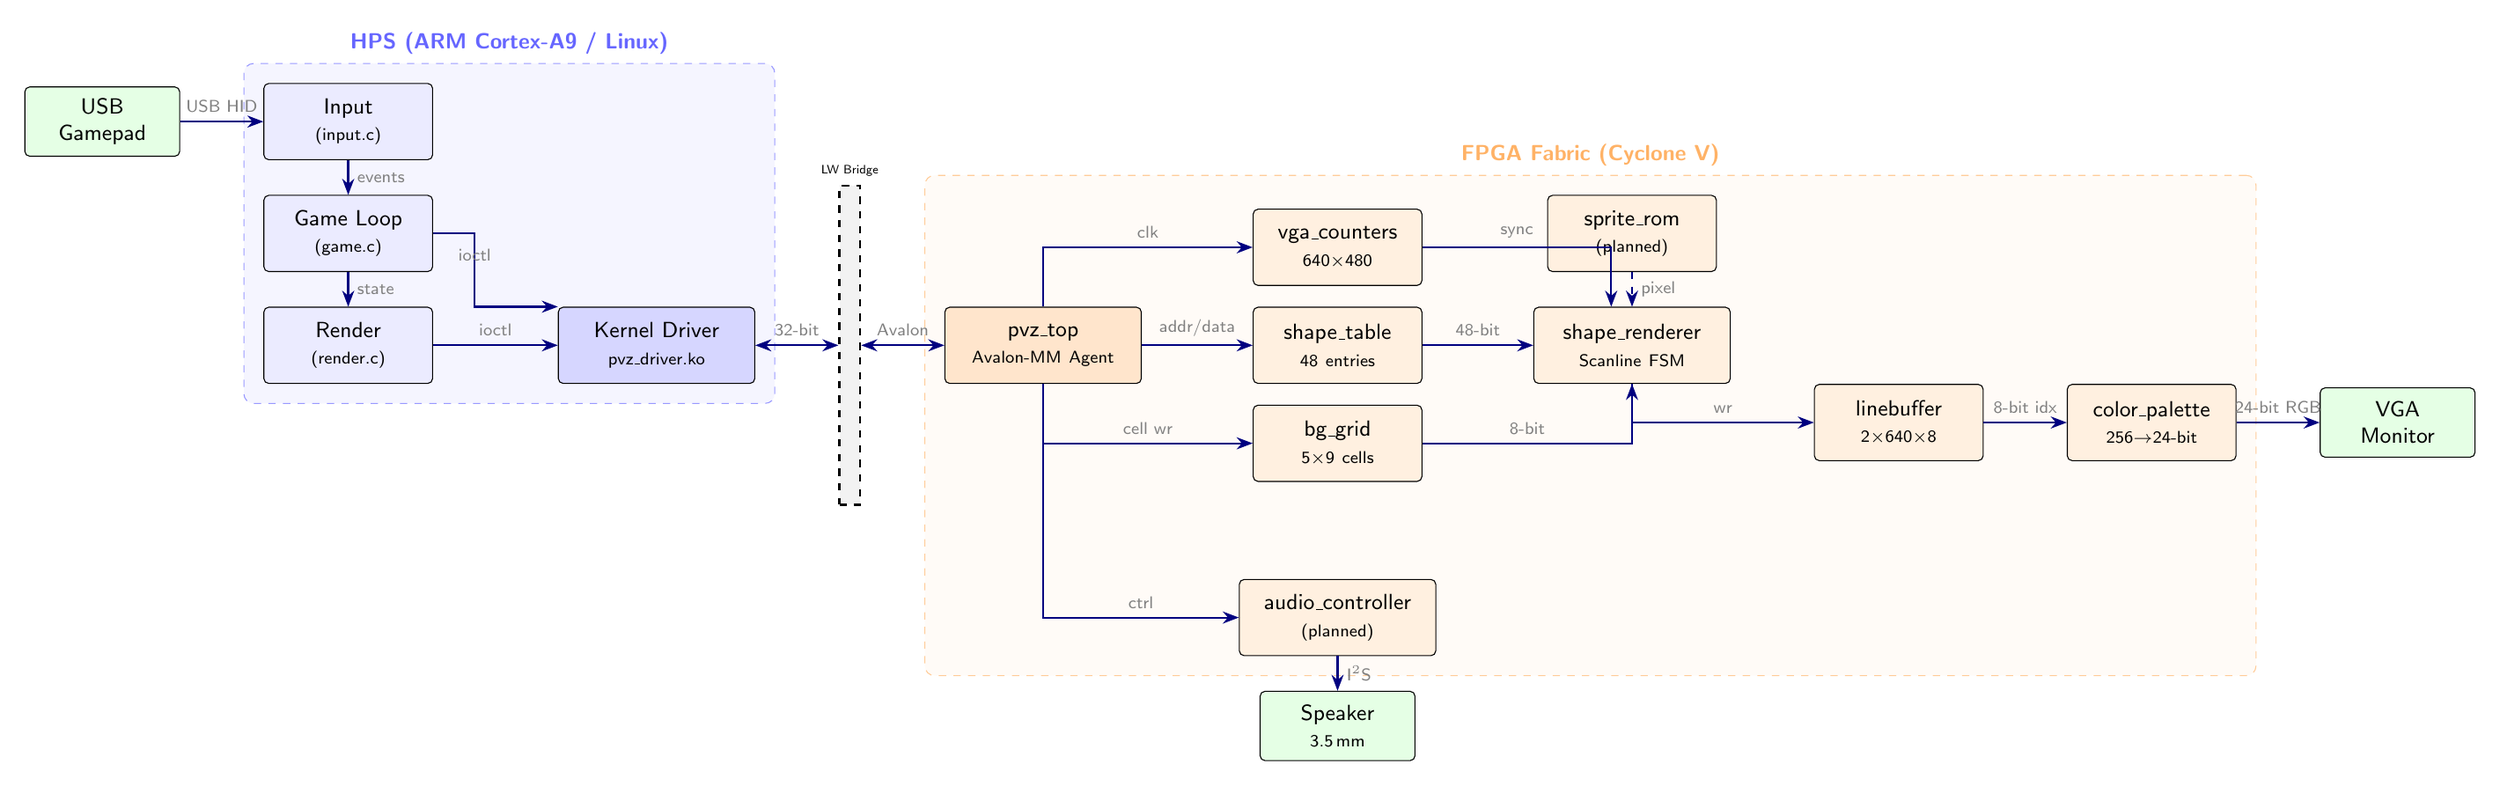
\begin{tikzpicture}[
  >=Stealth,
  block/.style={
    draw, rounded corners=2pt, minimum height=1.1cm,
    text width=2.4cm, align=center, font=\small\sffamily,
    fill=blue!8,
  },
  hwblock/.style={
    draw, rounded corners=2pt, minimum height=1.1cm,
    text width=2.4cm, align=center, font=\small\sffamily,
    fill=orange!12,
  },
  extblock/.style={
    draw, rounded corners=2pt, minimum height=1.0cm,
    text width=2.0cm, align=center, font=\small\sffamily,
    fill=green!10,
  },
  bus/.style={->, thick, color=NavyBlue},
  dbus/.style={<->, thick, color=NavyBlue},
  note/.style={font=\scriptsize\sffamily, color=gray},
]

% ── HPS Software ────────────────────────────────────────────────────
\node[block, text width=2.2cm] (gameloop)
  {Game Loop\\{\scriptsize(game.c)}};
\node[block, text width=2.2cm, below=0.5cm of gameloop] (render)
  {Render\\{\scriptsize(render.c)}};
\node[block, text width=2.2cm, above=0.5cm of gameloop] (input)
  {Input\\{\scriptsize(input.c)}};

% Kernel driver
\node[block, right=1.8cm of render, fill=blue!16, text width=2.6cm] (driver)
  {Kernel Driver\\{\scriptsize pvz\_driver.ko}};

% ── Bridge ──────────────────────────────────────────────────────────
\node[draw, thick, dashed, minimum height=4.6cm, minimum width=0.3cm,
      right=1.2cm of driver, fill=gray!10, label={[font=\tiny\sffamily]above:LW Bridge}]
      (bridge) {};

% ── FPGA blocks ─────────────────────────────────────────────────────
\node[hwblock, right=1.2cm of bridge, text width=2.6cm, fill=orange!20] (pvztop)
  {pvz\_top\\{\scriptsize Avalon-MM Agent}};

\node[hwblock, above right=0.3cm and 1.6cm of pvztop, text width=2.2cm] (vgacnt)
  {vga\_counters\\{\scriptsize 640$\times$480}};
\node[hwblock, right=1.6cm of pvztop, text width=2.2cm] (shapetbl)
  {shape\_table\\{\scriptsize 48 entries}};
\node[hwblock, below right=0.3cm and 1.6cm of pvztop, text width=2.2cm] (bggrid)
  {bg\_grid\\{\scriptsize 5$\times$9 cells}};

\node[hwblock, right=1.6cm of shapetbl, text width=2.6cm] (renderer)
  {shape\_renderer\\{\scriptsize Scanline FSM}};

\node[hwblock, above=0.5cm of renderer, text width=2.2cm] (spriterom)
  {sprite\_rom\\{\scriptsize (planned)}};

\node[hwblock, below right=0.0cm and 1.2cm of renderer, text width=2.2cm] (linebuf)
  {linebuffer\\{\scriptsize 2$\times$640$\times$8}};
\node[hwblock, right=1.2cm of linebuf, text width=2.2cm] (palette)
  {color\_palette\\{\scriptsize 256$\to$24-bit}};

\node[hwblock, below=1.4cm of bggrid, text width=2.6cm] (audioctrl)
  {audio\_controller\\{\scriptsize (planned)}};

% ── External peripherals ────────────────────────────────────────────
\node[extblock, right=1.2cm of palette] (vga) {VGA\\Monitor};
\node[extblock, left=1.2cm of input]    (gamepad) {USB\\Gamepad};
\node[extblock, below=0.5cm of audioctrl] (speaker) {Speaker\\{\scriptsize 3.5\,mm}};

% ── Connections: HPS ────────────────────────────────────────────────
\draw[bus] (input) -- (gameloop) node[midway,right,note] {events};
\draw[bus] (gameloop) -- (render) node[midway,right,note] {state};
\draw[bus] (render) -- (driver) node[midway,above,note] {ioctl};
\draw[bus] (gameloop.east) -| ([xshift=0.6cm]gameloop.east) |- (driver.north west)
           node[near start,above,note] {ioctl};
\draw[bus] (gamepad) -- (input) node[midway,above,note] {USB HID};

% ── Connections: Bridge ─────────────────────────────────────────────
\draw[dbus] (driver) -- (bridge) node[midway,above,note] {32-bit};
\draw[dbus] (bridge) -- (pvztop) node[midway,above,note] {Avalon};

% ── Connections: FPGA ───────────────────────────────────────────────
\draw[bus] (pvztop) -- (shapetbl) node[midway,above,note] {addr/data};
\draw[bus] (pvztop) |- (bggrid) node[near end,above,note] {cell wr};
\draw[bus] (pvztop) |- (vgacnt) node[near end,above,note] {clk};
\draw[bus] (pvztop) |- (audioctrl) node[near end,above,note] {ctrl};

\draw[bus] (shapetbl) -- (renderer) node[midway,above,note] {48-bit};
\draw[bus] (bggrid) -| (renderer) node[near start,above,note] {8-bit};
\draw[bus] (vgacnt) -| ([xshift=-0.3cm]renderer.north) node[near start,above,note] {sync};
\draw[bus, dashed] (spriterom) -- (renderer) node[midway,right,note] {pixel};

\draw[bus] (renderer) |- (linebuf) node[near end,above,note] {wr};
\draw[bus] (linebuf) -- (palette) node[midway,above,note] {8-bit idx};
\draw[bus] (palette) -- (vga) node[midway,above,note] {24-bit RGB};
\draw[bus] (audioctrl) -- (speaker) node[midway,right,note] {I$^2$S};

% ── Region labels ──────────────────────────────────────────────────
\begin{scope}[on background layer]
  \node[draw=blue!40, fill=blue!4, dashed, rounded corners=4pt,
        fit=(input)(gameloop)(render)(driver),
        inner sep=8pt, label={[font=\small\sffamily\bfseries,blue!60]above:HPS (ARM Cortex-A9 / Linux)}] {};
  \node[draw=orange!40, fill=orange!3, dashed, rounded corners=4pt,
        fit=(pvztop)(vgacnt)(shapetbl)(bggrid)(renderer)(linebuf)(palette)(spriterom)(audioctrl),
        inner sep=8pt, label={[font=\small\sffamily\bfseries,orange!60]above:FPGA Fabric (Cyclone V)}] {};
\end{scope}

\end{tikzpicture}%
}
\caption{System block diagram. Solid arrows show data flow; dashed
  blocks indicate planned modules not yet implemented. The lightweight
  HPS-to-FPGA bridge carries 32-bit Avalon-MM transactions between the
  kernel driver and the \texttt{pvz\_top} peripheral.}
\label{fig:system-block}
\end{figure}

\subsection{Module Summary}

Table~\ref{tab:modules} lists every hardware module, its role, and key
parameters.

\begin{table}[H]
\centering
\caption{FPGA module inventory.}
\label{tab:modules}
\begin{tabularx}{\textwidth}{l l X}
\toprule
\textbf{Module} & \textbf{Type} & \textbf{Description} \\
\midrule
\texttt{pvz\_top}        & Avalon-MM agent
  & Top-level peripheral.\ Decodes five 32-bit registers on the lightweight
    bridge and wires every sub-module together. \\
\texttt{vga\_counters}   & Timing gen.
  & Produces \texttt{hcount} (0--1599) and \texttt{vcount} (0--524) for
    640$\times$480 @ 60\,Hz from the 50\,MHz board clock. \\
\texttt{linebuffer}      & Dual SRAM
  & Two 640$\times$8-bit banks.\ One is read for display while the other
    accepts writes from the renderer; roles swap every hsync. \\
\texttt{bg\_grid}        & Grid LUT
  & Holds a per-cell palette index for the $5 \times 9$ game board.
    Shadow/active double-buffered at vsync. \\
\texttt{shape\_table}    & Entry store
  & 48-entry table, each 48~bits.\ CPU writes go to a shadow copy that
    latches to the active copy at vsync. \\
\texttt{shape\_renderer} & Scanline FSM
  & Fills the draw line buffer each scanline: background first, then
    overlays all visible shapes using a painter's-algorithm pass. \\
\texttt{color\_palette}  & LUT (comb.)
  & 256-entry lookup from 8-bit index to 24-bit RGB.  Purely
    combinational; no BRAM consumed. \\
\texttt{sprite\_rom}     & Block RAM
  & \emph{Planned.}\ Bitmap pixel data for plants, zombies, and UI
    elements. Indexed by sprite ID and sub-pixel offset. \\
\texttt{audio\_controller} & I$^2$S / I$^2$C
  & \emph{Planned.}\ Configures the WM8731 codec over I$^2$C and streams
    PCM samples from an on-chip wave ROM. \\
\bottomrule
\end{tabularx}
\end{table}

% ════════════════════════════════════════════════════════════════════════
\section{Algorithms}
\label{sec:algorithms}

\subsection{Game Loop (Software)}
\label{sec:algo-gameloop}

The main program runs a fixed-rate 60\,Hz loop on the HPS. Each frame
follows the sequence shown in Algorithm~\ref{alg:mainloop}. Frame pacing
uses \texttt{gettimeofday()} to measure elapsed time and sleeps for the
remainder of the 16.67\,ms budget.

\begin{figure}[H]
\begin{lstlisting}[
  language={},
  morekeywords={function,for,if,else,while,return,each,end,do},
  caption={Main game loop (60\,Hz).},
  label={alg:mainloop},
]
function main_loop():
    game_init()
    while state == PLAYING do
        t0 = current_time()

        // 1. Input
        key = input_poll()            // non-blocking USB/keyboard read
        handle_input(key)             // move cursor, place/remove plant

        // 2. Update game state
        update_sun()                  // +25 sun every 10 s
        update_spawning()             // wave-table-driven zombie spawns
        update_plant_firing()         // peashooters fire every 1.5 s
        update_projectiles()          // peas move right at 2 px/frame
        update_zombies()              // zombies move left; eat plants
        check_collisions()            // pea-zombie, zombie-plant
        check_win_lose()              // all waves cleared? zombie at x=0?

        // 3. Render
        render_background()           // ioctl: BG_CELL for each grid cell
        render_plants()               // ioctl: shape/sprite per plant
        render_zombies()              // ioctl: shape/sprite per zombie
        render_projectiles()          // ioctl: shape/sprite per pea
        render_hud()                  // sun counter, wave indicator
        commit_shapes()               // ioctl: SHAPE_COMMIT

        // 4. Pace
        dt = current_time() - t0
        sleep(16667 us - dt)
    end
\end{lstlisting}
\end{figure}

\subsubsection{Collision Detection}

Collision checks run in software every frame. Two kinds of overlap
matter:

\begin{enumerate}[nosep]
  \item \textbf{Pea--Zombie.}\  A pea and a zombie collide when they
    occupy the same row and their bounding boxes overlap horizontally:
    \[
      \text{pea}_x + \text{pea}_w \geq \text{zombie}_x
      \;\;\wedge\;\;
      \text{pea}_x \leq \text{zombie}_x + \text{zombie}_w.
    \]
    On collision the pea is removed and the zombie loses 1~HP.

  \item \textbf{Zombie--Plant.}\  A zombie's bounding box overlaps a
    grid cell when the zombie's left edge enters the cell's pixel region.
    The zombie then stops walking and instead deals damage over time to
    the plant until it is destroyed.
\end{enumerate}

\subsubsection{Sun Economy}

The player starts with 150~sun. A background timer adds 25~sun every
10~seconds. Sunflower plants accelerate income by producing 25~sun
every 10~seconds each. Placing a plant deducts its cost; the game
refuses the placement when the player cannot afford it.

\subsubsection{Wave System}

Zombie spawns follow a table stored in software. Each entry specifies a
time offset (in frames) and a zombie type. The table grows harder over
successive waves by introducing Conehead and Buckethead zombies and by
decreasing the gap between spawns.

% ────────────────────────────────────────────────────────────────────────
\subsection{VGA Rendering Pipeline (Hardware)}
\label{sec:algo-vga}

The display engine produces pixels one scanline at a time using dual
line buffers. While the VGA DAC reads from buffer~A, the renderer fills
buffer~B with the next line's pixel data. The two swap roles at every
horizontal sync pulse. This avoids the memory cost of a full frame
buffer (307\,KB at 8-bit color) and instead requires only
$2 \times 640 = 1{,}280$~bytes.

\subsubsection{Timing}

The \texttt{vga\_counters} module divides the 50\,MHz board clock by two
to produce a 25\,MHz pixel clock. Table~\ref{tab:vga-timing} lists the
timing parameters.

\begin{table}[H]
\centering
\caption{VGA 640$\times$480 @ 60\,Hz timing parameters.}
\label{tab:vga-timing}
\begin{tabular}{l r r l}
\toprule
\textbf{Parameter}   & \textbf{Pixels/Lines} & \textbf{Clocks (50\,MHz)} & \textbf{Notes} \\
\midrule
H Active             & 640 px    & 1280  & Visible pixels \\
H Front Porch        & 16 px     & 32    & \\
H Sync Pulse         & 96 px     & 192   & Active low \\
H Back Porch         & 48 px     & 96    & \\
\textbf{H Total}     & \textbf{800 px} & \textbf{1600} & \\
\midrule
V Active             & 480 lines & ---   & Visible lines \\
V Front Porch        & 10 lines  & ---   & \\
V Sync Pulse         & 2 lines   & ---   & Active low \\
V Back Porch         & 33 lines  & ---   & \\
\textbf{V Total}     & \textbf{525 lines} & --- & \\
\midrule
\textbf{Frame Rate}  & \multicolumn{2}{c}{$50\text{M} / (1600 \times 525) \approx 59.5$\,Hz} & \\
\bottomrule
\end{tabular}
\end{table}

\subsubsection{Scanline Rendering Sequence}

Figure~\ref{fig:scanline-timing} illustrates the per-scanline timing.
Three control signals derived from \texttt{hcount} and \texttt{vcount}
govern the pipeline:

\begin{itemize}[nosep]
  \item \textbf{\texttt{lb\_swap}} fires at \texttt{hcount\,=\,0} for
    each active line, toggling which buffer the DAC reads from.
  \item \textbf{\texttt{render\_start}} fires at \texttt{hcount\,=\,2},
    kicking off the renderer's FSM for the \emph{current} scanline.
  \item \textbf{\texttt{vsync\_latch}} fires once per frame at
    \texttt{vcount\,=\,480, hcount\,=\,0}, copying all shadow registers
    to their active counterparts.
\end{itemize}

\begin{figure}[H]
\centering
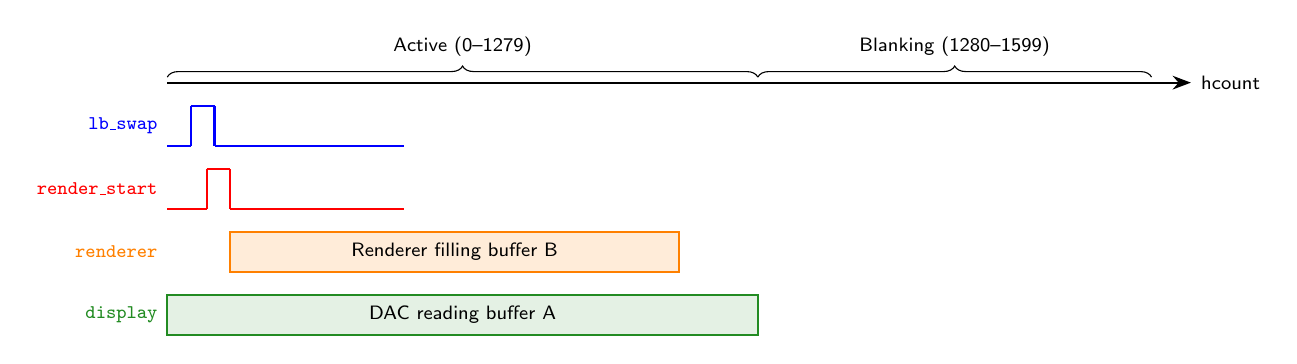
\begin{tikzpicture}[
  >=Stealth,
  sig/.style={thick},
  label/.style={font=\scriptsize\sffamily},
]
  % Time axis
  \draw[->, thick] (0,0) -- (13,0) node[right,label] {hcount};
  % Regions
  \draw[decorate, decoration={brace, amplitude=4pt, raise=2pt}]
    (0,0) -- (7.5,0) node[midway, above=6pt, label] {Active (0--1279)};
  \draw[decorate, decoration={brace, amplitude=4pt, raise=2pt}]
    (7.5,0) -- (12.5,0) node[midway, above=6pt, label] {Blanking (1280--1599)};

  % lb_swap pulse
  \draw[sig, blue] (0,-0.8) -- (0.3,-0.8);
  \draw[sig, blue] (0.3,-0.8) -- (0.3,-0.3);
  \draw[sig, blue] (0.3,-0.3) -- (0.6,-0.3);
  \draw[sig, blue] (0.6,-0.3) -- (0.6,-0.8);
  \draw[sig, blue] (0.6,-0.8) -- (3,-0.8);
  \node[left, label, blue] at (0,-0.55) {\texttt{lb\_swap}};

  % render_start pulse
  \draw[sig, red] (0,-1.6) -- (0.5,-1.6);
  \draw[sig, red] (0.5,-1.6) -- (0.5,-1.1);
  \draw[sig, red] (0.5,-1.1) -- (0.8,-1.1);
  \draw[sig, red] (0.8,-1.1) -- (0.8,-1.6);
  \draw[sig, red] (0.8,-1.6) -- (3,-1.6);
  \node[left, label, red] at (0,-1.35) {\texttt{render\_start}};

  % Renderer active
  \draw[sig, orange, fill=orange!15]
    (0.8,-2.4) rectangle (6.5,-1.9);
  \node[label] at (3.65,-2.15) {Renderer filling buffer B};
  \node[left, label, orange] at (0,-2.15) {\texttt{renderer}};

  % Display read
  \draw[sig, ForestGreen, fill=ForestGreen!12]
    (0,-3.2) rectangle (7.5,-2.7);
  \node[label] at (3.75,-2.95) {DAC reading buffer A};
  \node[left, label, ForestGreen] at (0,-2.95) {\texttt{display}};

\end{tikzpicture}
\caption{Per-scanline timing. The renderer has roughly 1\,598 clock
  cycles to fill the draw buffer before the next swap.}
\label{fig:scanline-timing}
\end{figure}

\subsubsection{Renderer FSM}

The \texttt{shape\_renderer} walks through six states each scanline:

\begin{enumerate}[nosep]
  \item \textbf{S\_IDLE} --- Waits for \texttt{render\_start}.
  \item \textbf{S\_BG\_FILL} --- Writes 640 pixels of background color
    from \texttt{bg\_grid} (one clock per pixel).
  \item \textbf{S\_SHAPE\_SETUP} --- Indexes the shape table, latches
    geometry into local registers.
  \item \textbf{S\_SHAPE\_CHECK} --- Tests whether the shape's vertical
    extent intersects the current scanline. If not, skips to the next
    shape.
  \item \textbf{S\_SHAPE\_DRAW} --- Iterates pixel-by-pixel across the
    shape's horizontal span, performing a type-dependent hit test
    (rectangle, circle, or 7-segment digit) and writing hits into the
    line buffer. Later shapes overwrite earlier ones, implementing
    painter's-algorithm z-ordering.
  \item \textbf{S\_DONE} --- Signals completion; idles until the next
    \texttt{render\_start}.
\end{enumerate}

Steps 3--5 repeat for all 48 shape entries.

% ────────────────────────────────────────────────────────────────────────
\subsection{Shape Types}
\label{sec:algo-shapes}

The renderer supports three shape primitives, selected by a 2-bit type
field:

\begin{description}[nosep, leftmargin=1.5cm, style=nextline]
  \item[Type 0 --- Filled Rectangle]
    Every pixel within the bounding box is a hit. This is the
    default for plants, zombies, grid cursor, and HUD backgrounds.

  \item[Type 1 --- Filled Circle]
    The hit test computes the squared distance from the pixel to the
    shape's center and compares it to the squared radius:
    \[
      (x - c_x)^2 + (y - c_y)^2 \;\leq\; \left(\tfrac{w}{2}\right)^2,
    \]
    where $c_x = s_x + w/2$ and $c_y = s_y + h/2$. This is used for pea
    projectiles.

  \item[Type 2 --- 7-Segment Digit]
    A hardcoded $20 \times 30$ pixel font with 3-pixel-thick segments.
    The digit value (0--9) is stored in bits $[3{:}0]$ of the width
    field. A combinational decoder maps each value to a 7-bit segment
    mask, and the hit test checks whether the local $(x, y)$ coordinate
    falls inside any active segment. This is used for the sun counter
    display.
\end{description}

% ────────────────────────────────────────────────────────────────────────
\subsection{Sprite System (Planned)}
\label{sec:algo-sprites}

The shape-based renderer described above serves the MVP. For the final
version we plan to add bitmap sprite support. Each sprite table entry
will gain a \texttt{sprite\_id} field that indexes into a block-RAM
sprite ROM. During the draw phase, instead of performing a geometric hit
test, the renderer will read pixel data from the ROM at the
corresponding $(x, y)$ offset. Palette index~0 means transparent, so
sprites with irregular outlines layer over the background without
rectangular halos.

Sprite sheets will be organized by entity type. Each sheet packs
multiple animation frames for one character (e.g., four walking frames
and two attack frames for the Peashooter). The sprite table entry's
\texttt{frame} field will select which animation frame to display.

% ────────────────────────────────────────────────────────────────────────
\subsection{Audio Playback (Planned)}
\label{sec:algo-audio}

The Wolfson WM8731 codec on the DE1-SoC accepts I$^2$S serial audio
data and provides analog output through the 3.5\,mm jack.

\textbf{Configuration.}\ At boot, software writes a sequence of register
values over the I$^2$C bus to set the codec's sample rate (8\,kHz),
word length (16-bit), and enable the DAC output path.

\textbf{Playback.}\ A hardware audio controller reads PCM samples from
an on-chip wave ROM and feeds them to the codec at the configured sample
rate. The wave ROM holds a looping background track and a handful of
short sound-effect clips. Software selects which clip to play by writing
a start address and length to audio control registers; the controller
then streams from that region, mixing it with the background track by
clamping the sum of the two sample values.

% ════════════════════════════════════════════════════════════════════════
\section{Entity Design}
\label{sec:entities}

\subsection{Plants}

Three plant types are planned. Table~\ref{tab:plants} lists their
properties.

\begin{table}[H]
\centering
\caption{Plant types and properties.}
\label{tab:plants}
\begin{tabular}{l r r l}
\toprule
\textbf{Plant} & \textbf{Sun Cost} & \textbf{HP (relative)} & \textbf{Behavior} \\
\midrule
Peashooter & 100 & $1\times$  & Fires a pea down its row every 1.5\,s \\
Sunflower  &  50 & $1\times$  & Produces 25 sun every 10\,s \\
Wall-nut   &  50 & $4\times$  & Absorbs damage; no attack \\
\bottomrule
\end{tabular}
\end{table}

\subsection{Zombies}

Three zombie types differ mainly in durability. All move leftward at the
same speed and eat any plant they reach.

\begin{table}[H]
\centering
\caption{Zombie types and properties.}
\label{tab:zombies}
\begin{tabular}{l r l}
\toprule
\textbf{Zombie} & \textbf{HP (relative)} & \textbf{Notes} \\
\midrule
Basic      & $1\times$  & Goes down quickly \\
Conehead   & $2\times$  & Traffic cone absorbs extra hits \\
Buckethead & $4\times$  & Highest durability \\
\bottomrule
\end{tabular}
\end{table}

\subsection{Projectiles}

Peashooters fire pea projectiles that travel rightward at approximately
120\,px/s (2~pixels per frame at 60\,fps). Each pea deals 1~HP of
damage on contact with a zombie and is then removed.

\subsection{Sun Economy}

\begin{itemize}[nosep]
  \item Starting sun: 150
  \item Passive income: $+25$ sun every 10\,s
  \item Sunflower bonus: additional $+25$ sun per Sunflower per 10\,s
  \item Maximum sun: capped (exact value TBD; bounds sprite table usage)
\end{itemize}

% ════════════════════════════════════════════════════════════════════════
\section{Resource Budgets}
\label{sec:resources}

The DE1-SoC's Cyclone~V 5CSEMA5F31C6 provides 4{,}450~Kbits of embedded
memory (M10K blocks), 32{,}070~ALMs, and 87~DSP blocks. This section
estimates our consumption of each.

\subsection{Graphics Memory}

Table~\ref{tab:gfx-mem} breaks down sprite storage. All sprites use
8-bit indexed color.

\begin{table}[H]
\centering
\caption{Graphics memory budget (8-bit indexed color).}
\label{tab:gfx-mem}
\begin{tabular}{l r r r r}
\toprule
\textbf{Category} & \textbf{Size (px)} & \textbf{Frames} & \textbf{Bits/sprite} & \textbf{Total (bits)} \\
\midrule
Peashooter       & $48\times48$ & 4 & 18{,}432 &  73{,}728 \\
Sunflower        & $48\times48$ & 4 & 18{,}432 &  73{,}728 \\
Wall-nut         & $48\times48$ & 2 & 18{,}432 &  36{,}864 \\
Basic Zombie     & $48\times64$ & 4 & 24{,}576 &  98{,}304 \\
Conehead Zombie  & $48\times64$ & 4 & 24{,}576 &  98{,}304 \\
Buckethead Zombie& $48\times64$ & 4 & 24{,}576 &  98{,}304 \\
Pea projectile   & $12\times12$ & 1 &  1{,}152 &   1{,}152 \\
Sun drop         & $24\times24$ & 1 &  4{,}608 &   4{,}608 \\
Cursor highlight & $72\times80$ & 1 & 46{,}080 &  46{,}080 \\
Plant cards (UI) & $40\times50$ & 3 & 16{,}000 &  48{,}000 \\
Background tile  & $72\times80$ & 2 & 46{,}080 &  92{,}160 \\
Digit font (0--9)& $20\times30$ & 10&  4{,}800 &  48{,}000 \\
\midrule
\multicolumn{4}{r}{\textbf{Graphics total}} & \textbf{719{,}232} \\
\bottomrule
\end{tabular}
\end{table}

\subsection{Audio Memory}

\begin{table}[H]
\centering
\caption{Audio memory budget (16-bit PCM, 8\,kHz).}
\label{tab:audio-mem}
\begin{tabular}{l r r r r}
\toprule
\textbf{Clip} & \textbf{Duration (s)} & \textbf{$f_s$ (kHz)} & \textbf{Samples} & \textbf{Bits} \\
\midrule
Background music  & 15.0 & 8 & 120{,}000 & 1{,}920{,}000 \\
Pea fire          &  0.3 & 8 &   2{,}400 &    38{,}400 \\
Zombie groan      &  0.5 & 8 &   4{,}000 &    64{,}000 \\
Plant placement   &  0.3 & 8 &   2{,}400 &    38{,}400 \\
Game over         &  3.0 & 8 &  24{,}000 &   384{,}000 \\
Victory           &  3.0 & 8 &  24{,}000 &   384{,}000 \\
\midrule
\multicolumn{4}{r}{\textbf{Audio total}} & \textbf{2{,}828{,}800} \\
\bottomrule
\end{tabular}
\end{table}

\subsection{On-Chip SRAM Summary}

\begin{table}[H]
\centering
\caption{Total on-chip memory usage estimate.}
\label{tab:sram}
\begin{tabular}{l r l}
\toprule
\textbf{Component} & \textbf{Bits} & \textbf{Notes} \\
\midrule
Line buffers (2$\times$640$\times$8)   &    10{,}240 & Dual scanline buffers \\
Shape table (48 entries $\times$ 48)    &     2{,}304 & Shadow + active $= 4{,}608$ \\
Background grid (5$\times$9$\times$8)  &       360   & Shadow + active $= 720$ \\
Color palette (256$\times$24)           &     6{,}144 & Combinational LUT (no BRAM) \\
Sprite ROMs                             &   719{,}232 & See Table~\ref{tab:gfx-mem} \\
Audio wave ROM                          & 2{,}828{,}800 & See Table~\ref{tab:audio-mem} \\
\midrule
\textbf{Total}                          & \textbf{3{,}567{,}304} & \\
\textbf{Available (M10K)}              & \textbf{4{,}450{,}000} & \\
\textbf{Utilization}                    & \textbf{80.2\%} & \\
\bottomrule
\end{tabular}
\end{table}

We have roughly 880\,Kbits of headroom. If audio memory proves too
tight we can reduce the background music loop duration or drop the
sample rate to 4\,kHz, which would halve the audio footprint.

\subsection{Logic Utilization}

The shape renderer is the most logic-intensive module due to the
signed multipliers for the circle distance check ($11 \times 11$~bit
multiply, two per pixel). Quartus typically maps these onto DSP blocks
rather than fabric ALMs. We estimate:

\begin{itemize}[nosep]
  \item VGA counters + control: $\sim$150~ALMs
  \item Shape renderer FSM + multipliers: $\sim$800~ALMs + 4~DSP blocks
  \item Shape table + background grid: $\sim$200~ALMs
  \item Color palette LUT: $\sim$100~ALMs
  \item Avalon decode: $\sim$50~ALMs
  \item Audio controller (planned): $\sim$300~ALMs
\end{itemize}

Total estimated: $\sim$1{,}600~ALMs out of 32{,}070 available (5\%).
Logic is not a constraint for this design.

% ════════════════════════════════════════════════════════════════════════
\section{Hardware/Software Interface}
\label{sec:hwsw}

\subsection{System Architecture}

The custom \texttt{pvz\_top} peripheral connects to the HPS through
Platform Designer's lightweight HPS-to-FPGA bridge. The CPU sees the
peripheral's base address at \texttt{0xFF200000}. The Avalon bus uses
32-bit words internally, so \texttt{pvz\_top}'s \texttt{address} port
carries word offsets (0--4). The kernel driver accesses registers using
byte offsets: \texttt{iowrite32(val, base + 4*N)} for word~$N$.

All rendering-visible registers are \textbf{shadow/active
double-buffered}. Writes from the CPU land in shadow copies. At the
start of the vertical blanking interval (\texttt{vcount\,=\,480,
hcount\,=\,0}), every shadow register latches into its active
counterpart. This ensures the display never shows a partially updated
frame.

\subsection{Register Map}

Table~\ref{tab:regmap} specifies every register. All registers are
\textbf{write-only} from the CPU side.

\begin{table}[H]
\centering
\caption{Avalon-MM register map (32-bit words, byte offsets).}
\label{tab:regmap}
\small
\begin{tabular}{c l c l l}
\toprule
\textbf{Offset} & \textbf{Name} & \textbf{Bits} & \textbf{Field} & \textbf{Description} \\
\midrule
\multirow{3}{*}{\texttt{0x00}}
  & \multirow{3}{*}{BG\_CELL}
  & $[2{:}0]$   & \texttt{col}   & Grid column (0--8) \\
  & & $[4{:}3]$   & \texttt{row}   & Grid row (0--4) \\
  & & $[15{:}8]$  & \texttt{color} & Palette index for this cell \\
\midrule
\texttt{0x04}
  & SHAPE\_ADDR
  & $[5{:}0]$   & \texttt{index} & Shape entry to modify (0--47) \\
\midrule
\multirow{4}{*}{\texttt{0x08}}
  & \multirow{4}{*}{SHAPE\_DATA0}
  & $[1{:}0]$   & \texttt{type}    & 0\,=\,rect, 1\,=\,circle, 2\,=\,7-seg \\
  & & $[2]$       & \texttt{visible} & 1\,=\,draw, 0\,=\,skip \\
  & & $[12{:}3]$  & \texttt{x}       & X position in pixels (0--639) \\
  & & $[21{:}13]$ & \texttt{y}       & Y position in pixels (0--479) \\
\midrule
\multirow{3}{*}{\texttt{0x0C}}
  & \multirow{3}{*}{SHAPE\_DATA1}
  & $[8{:}0]$   & \texttt{w}     & Width in pixels; or digit value $[3{:}0]$ for type\,2 \\
  & & $[17{:}9]$  & \texttt{h}     & Height in pixels \\
  & & $[25{:}18]$ & \texttt{color} & Palette index for shape fill \\
\midrule
\texttt{0x10}
  & SHAPE\_COMMIT
  & $[0]$       & \texttt{commit}& Write 1 to commit entry to shadow table \\
\bottomrule
\end{tabular}
\end{table}

\subsubsection{Write Sequence}

To update a shape entry, the CPU performs four writes in order:

\begin{enumerate}[nosep]
  \item Write \texttt{SHAPE\_ADDR} with the entry index (0--47).
  \item Write \texttt{SHAPE\_DATA0} with type, visible, $x$, and $y$.
  \item Write \texttt{SHAPE\_DATA1} with $w$, $h$, and color.
  \item Write \texttt{SHAPE\_COMMIT} with any nonzero value.
\end{enumerate}

After step~4, the staging registers are copied into the shadow table at
the specified index. The entry becomes visible on screen at the next
vsync. Background cell writes (\texttt{BG\_CELL}) take effect
immediately in the shadow grid with no explicit commit step.

\subsection{Shape Table Entry Format}
\label{sec:shape-entry}

Each entry in the 48-deep shape table is stored as 48~bits, packed as
shown in Figure~\ref{fig:shape-bits}.

\begin{figure}[H]
\centering
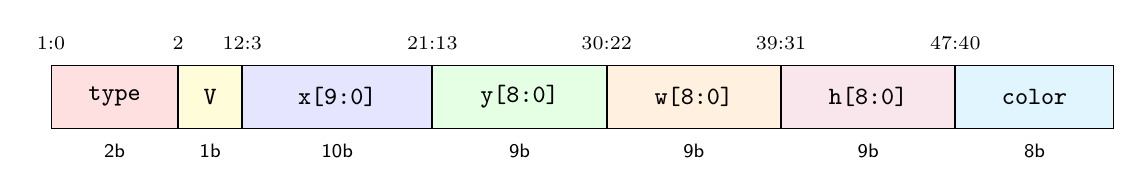
\begin{tikzpicture}[
  font=\small\ttfamily,
  box/.style={draw, minimum height=0.8cm, anchor=west},
]
  % Bit field boxes
  \node[box, fill=red!12,    minimum width=1.6cm] (type) at (0,0) {type};
  \node[box, fill=yellow!15, minimum width=0.8cm, right=0pt of type] (vis) {V};
  \node[box, fill=blue!10,   minimum width=2.4cm, right=0pt of vis]  (xf)  {x[9:0]};
  \node[box, fill=green!10,  minimum width=2.2cm, right=0pt of xf]   (yf)  {y[8:0]};
  \node[box, fill=orange!12, minimum width=2.2cm, right=0pt of yf]   (wf)  {w[8:0]};
  \node[box, fill=purple!10, minimum width=2.2cm, right=0pt of wf]   (hf)  {h[8:0]};
  \node[box, fill=cyan!12,   minimum width=2.0cm, right=0pt of hf]   (cf)  {color};

  % Bit numbers
  \node[above=2pt, font=\scriptsize] at (type.north west) {1:0};
  \node[above=2pt, font=\scriptsize] at (vis.north west) {2};
  \node[above=2pt, font=\scriptsize] at (xf.north west) {12:3};
  \node[above=2pt, font=\scriptsize] at (yf.north west) {21:13};
  \node[above=2pt, font=\scriptsize] at (wf.north west) {30:22};
  \node[above=2pt, font=\scriptsize] at (hf.north west) {39:31};
  \node[above=2pt, font=\scriptsize] at (cf.north west) {47:40};

  % Width labels
  \node[below=2pt, font=\scriptsize\sffamily] at (type.south) {2b};
  \node[below=2pt, font=\scriptsize\sffamily] at (vis.south)  {1b};
  \node[below=2pt, font=\scriptsize\sffamily] at (xf.south)   {10b};
  \node[below=2pt, font=\scriptsize\sffamily] at (yf.south)   {9b};
  \node[below=2pt, font=\scriptsize\sffamily] at (wf.south)   {9b};
  \node[below=2pt, font=\scriptsize\sffamily] at (hf.south)   {9b};
  \node[below=2pt, font=\scriptsize\sffamily] at (cf.south)   {8b};
\end{tikzpicture}
\caption{48-bit shape table entry layout. ``V'' is the visibility flag.}
\label{fig:shape-bits}
\end{figure}

\subsection{Planned Register Extensions}

The final version will add registers for sprite ROM access, audio
control, and frame synchronization:

\begin{table}[H]
\centering
\caption{Planned additional registers.}
\label{tab:planned-regs}
\begin{tabular}{c l l}
\toprule
\textbf{Offset} & \textbf{Name} & \textbf{Purpose} \\
\midrule
\texttt{0x14} & SPRITE\_ID     & Sprite ROM index for bitmap mode \\
\texttt{0x18} & SPRITE\_FRAME  & Animation frame selector \\
\texttt{0x1C} & AUDIO\_CTRL    & Start/stop BGM, trigger sound effect \\
\texttt{0x20} & AUDIO\_ADDR    & Wave ROM start address for sound effect \\
\texttt{0x24} & AUDIO\_LEN     & Sample count for sound effect clip \\
\texttt{0x28} & STATUS         & $[0]$: vsync flag (read-only), for frame sync \\
\bottomrule
\end{tabular}
\end{table}

\subsection{Kernel Driver Interface}
\label{sec:driver}

The Linux kernel module (\texttt{pvz\_driver.ko}) registers a misc
device at \texttt{/dev/pvz}. It matches the device tree compatible
string \texttt{csee4840,pvz\_gpu-1.0} generated by Platform Designer's
\texttt{\_hw.tcl} component descriptor. The driver exposes three
\texttt{ioctl} commands:

\begin{table}[H]
\centering
\caption{Kernel driver ioctl commands.}
\label{tab:ioctls}
\begin{tabular}{l l l}
\toprule
\textbf{ioctl} & \textbf{Argument} & \textbf{Action} \\
\midrule
\texttt{PVZ\_WRITE\_BG}
  & \texttt{pvz\_bg\_arg\_t}
  & Pack \texttt{col}, \texttt{row}, \texttt{color} into \texttt{BG\_CELL} \\
\texttt{PVZ\_WRITE\_SHAPE}
  & \texttt{pvz\_shape\_arg\_t}
  & Sequence: \texttt{ADDR} $\to$ \texttt{DATA0} $\to$ \texttt{DATA1} $\to$ \texttt{COMMIT} \\
\texttt{PVZ\_COMMIT\_SHAPES}
  & (none)
  & Reserved for batch-commit optimization \\
\bottomrule
\end{tabular}
\end{table}

The argument structures are:

\begin{lstlisting}[language=C, caption={Driver argument structures.}]
typedef struct {
    unsigned char col;    // 0-8
    unsigned char row;    // 0-4
    unsigned char color;  // palette index
} pvz_bg_arg_t;

typedef struct {
    unsigned char index;   // 0-47
    unsigned char type;    // 0=rect, 1=circle, 2=7seg
    unsigned char visible; // 0 or 1
    unsigned short x, y;   // pixel position
    unsigned short w, h;   // dimensions (or digit value for type 2)
    unsigned char color;   // palette index
} pvz_shape_arg_t;
\end{lstlisting}

\subsection{Platform Designer Integration}

Three artifacts must stay in sync whenever the peripheral changes:

\begin{enumerate}[nosep]
  \item \textbf{\texttt{pvz\_top.sv}} --- Verilog module ports and
    register decode logic.
  \item \textbf{\texttt{pvz\_top\_hw.tcl}} --- Platform Designer
    component descriptor. Sets the compatible string to
    \texttt{"csee4840,pvz\_gpu-1.0"} so the generated device tree
    includes the right node.
  \item \textbf{\texttt{pvz\_driver.c}} --- Kernel module whose
    \texttt{of\_device\_id} table matches that compatible string.
\end{enumerate}

If any one of these three diverges, the peripheral silently fails to
appear at boot. This kind of mismatch is easy to introduce and hard
to debug because nothing errors out---the device node just never shows
up.

\subsection{Color Palette}
\label{sec:palette}

The MVP palette is a small, hardcoded set of 13 colors (Table~\ref{tab:palette}).
The final version will expand this to cover all sprite artwork.

\begin{table}[H]
\centering
\caption{MVP color palette (8-bit index $\to$ 24-bit RGB).}
\label{tab:palette}
\begin{tabular}{c l c}
\toprule
\textbf{Index} & \textbf{Name} & \textbf{RGB (hex)} \\
\midrule
0  & Black        & \texttt{000000} \\
1  & Dark Green   & \texttt{1B5E20} \\
2  & Light Green  & \texttt{2D8B2D} \\
3  & Brown        & \texttt{8B4513} \\
4  & Yellow       & \texttt{FFD700} \\
5  & Red          & \texttt{FF0000} \\
6  & Dark Red     & \texttt{8B0000} \\
7  & Green        & \texttt{008000} \\
8  & Dark Green 2 & \texttt{006400} \\
9  & Bright Green & \texttt{00FF00} \\
10 & White        & \texttt{FFFFFF} \\
11 & Gray         & \texttt{808080} \\
12 & Orange       & \texttt{FFA500} \\
\bottomrule
\end{tabular}
\end{table}

% ════════════════════════════════════════════════════════════════════════
\section{Input System}
\label{sec:input}

The player uses a USB gamepad connected to the HPS. The game program
reads it through \texttt{libusb}, parsing USB HID reports for button and
D-pad state. A keyboard fallback reads from \texttt{/dev/input/eventX}
using non-blocking \texttt{read()} calls with \texttt{O\_NONBLOCK}.

\begin{table}[H]
\centering
\caption{Controller mapping.}
\label{tab:controls}
\begin{tabular}{l l l}
\toprule
\textbf{Button} & \textbf{Keyboard Fallback} & \textbf{Action} \\
\midrule
D-pad Up    & Arrow Up    & Move cursor up one row \\
D-pad Down  & Arrow Down  & Move cursor down one row \\
D-pad Left  & Arrow Left  & Move cursor left one column \\
D-pad Right & Arrow Right & Move cursor right one column \\
A           & Space       & Place selected plant at cursor \\
B           & D           & Remove plant / cancel selection \\
L/R         & (planned)   & Cycle plant type selection \\
Start       & Escape      & Quit game \\
\bottomrule
\end{tabular}
\end{table}

Input is polled once per frame (60\,Hz). Only key-down events are
processed; key repeats and releases are filtered out.

% ════════════════════════════════════════════════════════════════════════
\section{Display Layout}
\label{sec:display}

Figure~\ref{fig:screen-layout} shows how the 640$\times$480 screen is
divided.

\begin{figure}[H]
\centering
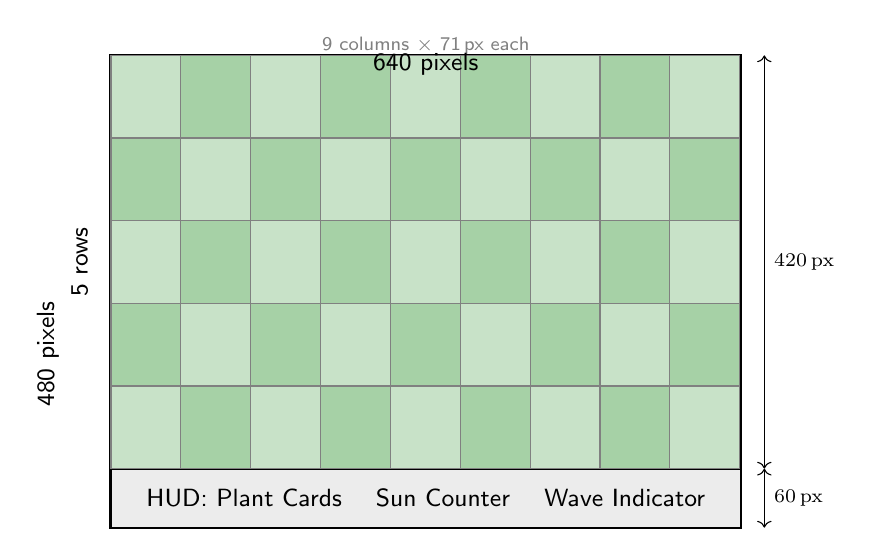
\begin{tikzpicture}[
  font=\small\sffamily,
  region/.style={draw, thick},
]
  % Scale: 1cm = 80px
  \def\sx{0.0125}  % x scale
  \def\sy{0.0125}  % y scale (inverted: 0 at top)

  % Screen outline
  \draw[very thick] (0,0) rectangle ({640*\sx},{480*\sy});

  % HUD region
  \draw[region, fill=gray!15]
    (0, 0) rectangle ({640*\sx}, {60*\sy});
  \node at ({320*\sx}, {30*\sy}) {HUD: Plant Cards \quad Sun Counter \quad Wave Indicator};

  % Grid region
  \foreach \r in {0,...,4} {
    \foreach \c in {0,...,8} {
      \pgfmathsetmacro{\x}{\c * 71 * \sx}
      \pgfmathsetmacro{\y}{(60 + \r * 84) * \sy}
      \pgfmathsetmacro{\w}{71 * \sx}
      \pgfmathsetmacro{\h}{84 * \sy}
      \pgfmathparse{mod(\r+\c,2) == 0 ? 1 : 0}
      \ifnum\pgfmathresult=1
        \fill[ForestGreen!25] (\x, \y) rectangle ({\x+\w}, {\y+\h});
      \else
        \fill[ForestGreen!40] (\x, \y) rectangle ({\x+\w}, {\y+\h});
      \fi
      \draw[thin, gray] (\x, \y) rectangle ({\x+\w}, {\y+\h});
    }
  }

  % Labels
  \node[rotate=90] at (-0.4, {(60+210)*\sy}) {\small 5 rows};
  \draw[<->] ({640*\sx + 0.3}, {60*\sy}) -- ({640*\sx + 0.3}, {60*\sy + 420*\sy})
    node[midway, right, font=\scriptsize] {420\,px};
  \draw[<->] ({640*\sx + 0.3}, 0) -- ({640*\sx + 0.3}, {60*\sy})
    node[midway, right, font=\scriptsize] {60\,px};

  % Bottom status
  \node at ({320*\sx}, {(60 + 420 + 10)*\sy})
    [font=\scriptsize\sffamily, text=gray] {9 columns $\times$ 71\,px each};

  % Dimension labels
  \node[below] at ({320*\sx}, {480*\sy + 0.15})
    {\small 640 pixels};
  \node[left, rotate=90] at (-0.8, {240*\sy})
    {\small 480 pixels};

\end{tikzpicture}
\caption{Screen layout. The top 60 pixels hold the HUD; the remaining
  420 pixels hold the $5 \times 9$ game grid (each cell approximately
  $71 \times 84$ pixels). The checkerboard pattern distinguishes
  alternating cells.}
\label{fig:screen-layout}
\end{figure}

Coordinate mapping from grid cell $(r, c)$ to pixel origin:
\[
  x = c \times 71, \qquad y = 60 + r \times 84.
\]

% ════════════════════════════════════════════════════════════════════════
\section{Testing and Verification}
\label{sec:testing}

\subsection{Hardware Testbenches}

\begin{itemize}[nosep]
  \item \textbf{VGA timing} --- Verify \texttt{hcount}/\texttt{vcount}
    ranges, sync pulse widths and polarities, and blanking intervals
    against the 640$\times$480 standard.
  \item \textbf{Linebuffer swap} --- Confirm that buffer roles toggle
    correctly on the \texttt{lb\_swap} pulse and that read and write
    ports never alias the same bank simultaneously.
  \item \textbf{Shape rendering} --- Feed known shape entries and
    compare the linebuffer contents against a golden reference computed
    in the testbench.
  \item \textbf{End-to-end} --- Simulate a full frame using Verilator,
    dump the pixel output to a PPM image, and visually inspect.
\end{itemize}

\subsection{Software Unit Tests}

A host-compilable test harness (\texttt{test/test\_game.c}) exercises
the game logic without any hardware dependency:

\begin{itemize}[nosep]
  \item Initial state validation (grid clear, sun = 150)
  \item Plant placement and sun deduction
  \item Sun auto-increment timing
  \item Pea--zombie collision detection
  \item Zombie destruction at 0~HP
  \item Lose condition (zombie at $x = 0$)
  \item Win condition (all zombies spawned and defeated)
\end{itemize}

\subsection{On-Board Integration}

\begin{itemize}[nosep]
  \item \textbf{\texttt{test\_shapes}} --- Writes a checkerboard
    background and several sample shapes via ioctl, confirming that the
    driver--hardware path works end to end.
  \item \textbf{\texttt{test\_input}} --- Polls
    \texttt{/dev/input/eventX} at 60\,Hz and prints recognized keys,
    verifying that the gamepad/keyboard input pipeline works.
\end{itemize}

% ════════════════════════════════════════════════════════════════════════

\end{document}
